\documentclass[ucs,10pt]{beamer}
 
% Template for talks using the Logo of STCE and Corporate Design of RWTH Aachen
% adapted from:
% https://www.mi.fu-berlin.de/w/Mi/BeamerTemplateCorporateDesign

\usepackage{amsmath,dsfont,listings}

%%% STCE logo
% small version for upper right corner of normal pages
\pgfdeclareimage[height=0.9cm]{university-logo}{rwth_i12_softw-werkz_en_rgb.png}
\logo{\pgfuseimage{university-logo}}
% large version for upper right corner of title page
\pgfdeclareimage[height=1cm]{big-university-logo}{rwth_i12_softw-werkz_en_rgb.png}
\newcommand{\titleimage}[1]{\pgfdeclareimage[height=2cm]{title-image}{#1}}
\titlegraphic{\pgfuseimage{title-image}}
%%% end STCE logo

% NOTE: 1cm = 0.393 in = 28.346 pt;    1 pt = 1/72 in = 0.0352 cm
\setbeamersize{text margin right=3.5mm, text margin left=7.5mm}  % text margin

% colors to be used
\definecolor{text-grey}{RGB}{51, 51, 51} % grey text on white background
\definecolor{bg-grey}{rgb}{0.66, 0.65, 0.60} % grey background (for white text)
\definecolor{rwth-blue}{RGB}{0, 83, 159} % blue text
\definecolor{rwth-green}{RGB}{153, 204, 0} % green text
\definecolor{rwth-red}{RGB}{204, 0, 0} % red text (used by \alert)

% switch off the sidebars
% TODO: loading \useoutertheme{sidebar} (which is maybe wanted) also inserts
%   a sidebar on title page (unwanted), also indents the page title (unwanted?),
%   and duplicates the navigation symbols (unwanted)
\setbeamersize{sidebar width left=0cm, sidebar width right=0mm}
\setbeamertemplate{sidebar right}{}
\setbeamertemplate{sidebar left}{}
%    XOR
% \useoutertheme{sidebar}

% frame title
% is truncated before logo and splits on two lines
% if neccessary (or manually using \\)
\setbeamertemplate{frametitle}{%
    \vskip-30pt \color{purple}\large%
    \begin{minipage}[b][23pt]{80.5mm}%
    \flushleft\insertframetitle%
    \end{minipage}%
}

%%% title page
% TODO: get rid of the navigation symbols on the title page.
%   actually, \frame[plain] *should* remove them...
\setbeamertemplate{title page}{
% upper right: STCE logo
\vskip2pt\hfill\pgfuseimage{big-university-logo} \\
\vskip6pt\hskip3pt
% title image of the presentation
% set the title and the author
\begin{center}
\vskip4pt
\large \inserttitle \vskip5pt  \small \insertsubtitle
\vskip8pt
	\normalsize \insertauthor %\\ 
	%\includegraphics[width=2cm]{../../foto_naumann}	
\\ [5mm]
	\footnotesize \insertinstitute 
\end{center}
}
%%% end title page

%%% colors
\usecolortheme{lily}
\setbeamercolor*{normal text}{fg=black,bg=white}
\setbeamercolor*{alerted text}{fg=rwth-red}
\setbeamercolor*{example text}{fg=rwth-green}
\setbeamercolor*{structure}{fg=rwth-blue}

\setbeamercolor*{block title}{fg=white,bg=black!50}
\setbeamercolor*{block title alerted}{fg=white,bg=black!50}
\setbeamercolor*{block title example}{fg=white,bg=black!50}

\setbeamercolor*{block body}{bg=black!10}
\setbeamercolor*{block body alerted}{bg=black!10}
\setbeamercolor*{block body example}{bg=black!10}

\setbeamercolor{bibliography entry author}{fg=rwth-blue}
% TODO: this doesn't work at all:
\setbeamercolor{bibliography entry journal}{fg=text-grey}

\setbeamercolor{item}{fg=rwth-blue}
\setbeamercolor{navigation symbols}{fg=text-grey,bg=bg-grey}
%%% end colors

%%% headline
\setbeamertemplate{headline}{
\vskip4pt\hfill\insertlogo\hspace{3.5mm} % logo on the right

\vskip6pt\color{rwth-blue}\rule{\textwidth}{0.4pt} % horizontal line
}
%%% end headline

%%% footline
\newcommand{\footlinetext}{\insertshortinstitute, \insertshorttitle}
\setbeamertemplate{footline}{
\vskip5pt\color{rwth-blue}\rule{\textwidth}{0.4pt}\\ % horizontal line
\vskip2pt
\makebox[123mm]{\hspace{7.5mm}
\color{rwth-blue}\footlinetext
\hfill \raisebox{-1pt}{\usebeamertemplate***{navigation symbols}}
\hfill \insertframenumber}
\vskip4pt
}
%%% end footline

%%% settings for listings package
\lstset{extendedchars=true, showstringspaces=false, basicstyle=\footnotesize\sffamily, tabsize=2, breaklines=true, breakindent=10pt, frame=l, columns=fullflexible}
\lstset{language=C++} % this sets the syntax highlighting
\lstset{mathescape=true} % this switches on $...$ substitution in code
% enables UTF-8 in source code:
\lstset{literate={ä}{{\"a}}1 {ö}{{\"o}}1 {ü}{{\"u}}1 {Ä}{{\"A}}1 {Ö}{{\"O}}1 {Ü}{{\"U}}1 {ß}{\ss}1}
%%% end listings
  

\begin{document}
\title[{\tt info@stce.rwth-aachen.de}]{\textcolor{rwth-blue}{Software Lab Computational Engineering Science} \vspace{.2cm} \\ {\small Group 12, Pusher Mechanism}}
\author[Group 12)]{Aaron Floerke, Arseniy Kholod, Xinyang Song and Yanliang Zhu} 
\institute[Software Lab CES]{
{Informatik 12: Software and Tools for Computational Engineering (STCE)} \\ RWTH Aachen University \vspace{.5cm}
}
\date[]{24.06.2024}



\begin{frame}[plain]
\titlepage
\end{frame}

\begin{frame}
	\frametitle{Contents}
\tableofcontents
\end{frame}



\section{Analysis}

\subsection{User Requirements}


\begin{frame}
\frametitle{Analysis \\
    \small \color{rwth-blue} User Requirements}
    \begin{itemize}
        \item Establish the basic geometry for a planar mechanism to achieve the given path.
        \item Provide the following data for the designed four-bar mechanism:
        \begin{itemize}
            \item Position of the two fixed pivot positions
            \item Lengths of the three moving links and of the fourth base link
            \item The position of the couple offset point relative to the coupler
        \end{itemize}
        \item Using Solid Edge, design and generate the 3D models of links of the mechanism:
        \begin{itemize}
            \item Construct the links out of sub-parts
            \item Assemble the links
            \item A diagram (produced from Solid Edge) of the assembled 3D mechanism
        \end{itemize}
        \item Simulate the motion of the mechanism using the Simply Motion option within Solid Edge.
        \item Evaluate the KE of the mechanism as it cycles:
        \begin{itemize}
            \item Produce a graph of the KE against time (or against crank angle) with at least 36 points
            \item Find the kinetic energy of the mechanism as it goes through a cycle
        \end{itemize}
        \item Obtain a configuration suitable for RP production.
    \end{itemize}
\end{frame}



\section{Essential Technical Background}

\begin{frame}
\frametitle{Essential Technical Background \\
    \small \color{rwth-blue} The Four Bar Mechanism}
    \begin{itemize}
        \item Online Demo: \url{https://www.geogebra.org/m/BueCG9ch}
        \item 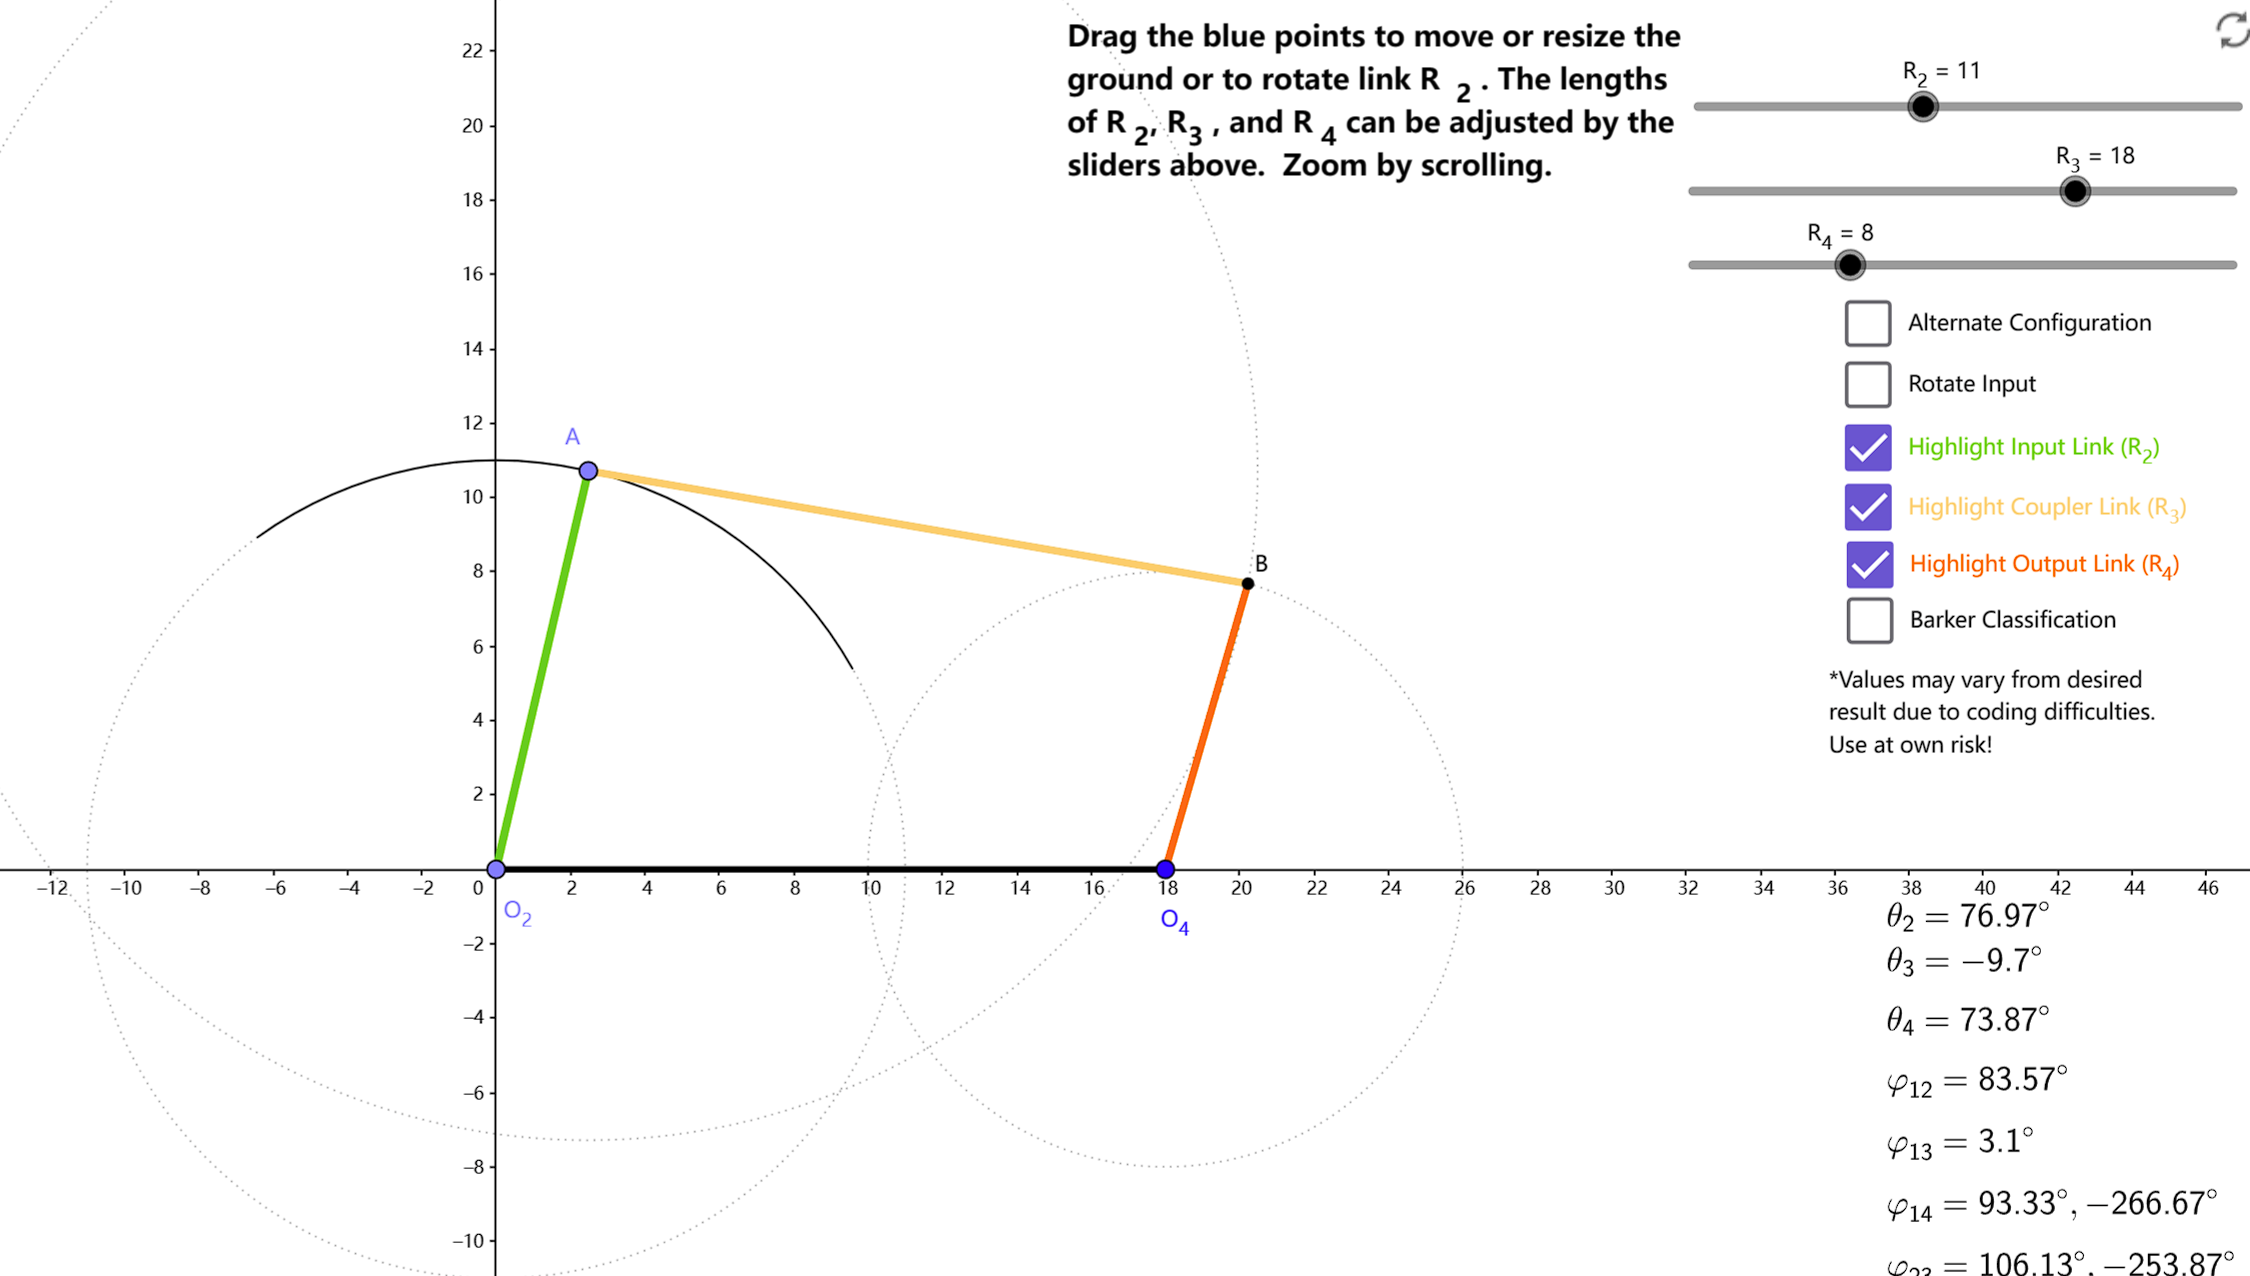
\includegraphics[width=\linewidth]{./Used_Picture/Online_Demo_1.png}
    \end{itemize}
\end{frame}


\begin{frame}
\frametitle{Essential Technical Background \\
	\small \color{rwth-blue} The Example}
	\begin{itemize}
        \item 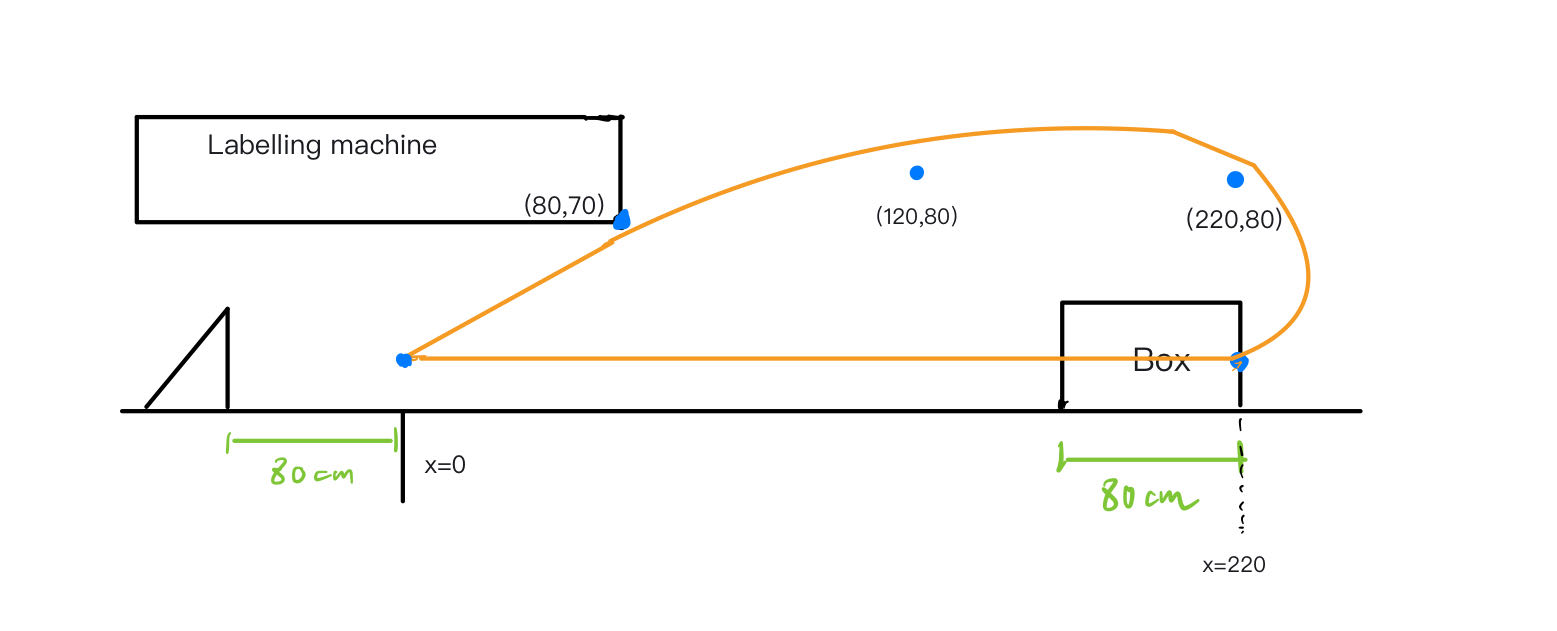
\includegraphics[width=\linewidth]{./Used_Picture/Example_1.jpg}
	\end{itemize}
\end{frame}


\subsection{System Requirements}

\begin{frame}
\frametitle{Analysis \\
    \small \color{rwth-blue} System Requirements}
    Functional:
    \begin{itemize}
        \item Use the "mechanism selector" in the constraint modeller to find a four-bar mechanism that fits the given path.
        \item Use the CAD (Solid Edge) to generate parts as 3D models:
        \begin{itemize}
            \item Construct the links out of sub-parts (to minimize the eventual cost of RP).
            \item Assemble the links in Solid Edge to ensure that they fit together.
            \item Additional requirements for RP:
            \begin{itemize}
                \item Moving parts should be designed with a clearance between holes and shafts of approximately 0.25mm.
            \end{itemize}
        \end{itemize}
        \item Simulate the motion of the mechanism using the Simply Motion option within Solid Edge.
    \end{itemize}
\end{frame}


\begin{frame}
\frametitle{Analysis \\
    \small \color{rwth-blue} System Requirements}
    Functional:
    \begin{itemize}
        \item Evaluate the KE of the mechanism as it cycles:
        \begin{itemize}
            \item Use the constraint modeller or other appropriate methods:
            \begin{itemize}
                \item Firstly adapt a macro for a four-bar chain to represent and simulate the motion of the particular mechanism.
                \item Then enhance the macro to find velocities and kinetic energies of the links.
            \end{itemize}
            \item Results to be achieved:
            \begin{itemize}
                \item Produce a graph of the KE against time (or against crank angle) with at least 36 points.
                \item Find the kinetic energy of the mechanism as it goes through a cycle.
            \end{itemize}
        \end{itemize}
        \item Obtain a configuration suitable for RP production:
        \begin{itemize}
            \item In Solid Edge, save each component as a separate part file.
            \item Lay out the various parts using Solid Edge on a plane.
            \item These parts then need to be packed reasonably closely on a plane region of size 140mm x 220mm.
            \item Identify the maximum height (RP build depth).
        \end{itemize}
    \end{itemize}
\end{frame}

\begin{frame}
\frametitle{Analysis \\
    \small \color{rwth-blue} System Requirements}
    Non-Functional:
    \begin{itemize}
        \item Use the constraint modelling software created at Bath University.
        \item Use Solid Edge.
        \item Provide the following data for the designed four-bar mechanism:
        \begin{itemize}
            \item Position of the two fixed pivot positions.
            \item Lengths of the three moving links and of the fourth base link.
            \item The position of the couple offset point relative to the coupler.
        \end{itemize}
        \item Things to be prepared:
        \begin{itemize}
            \item A listing of any constraint modeller macro used.
            \item A listing of any programming language code used.
            \item An indication of the calculation performed by any spreadsheet used.
            \item The graph of KE and a statement of its maximum value.
        \end{itemize}
    \end{itemize}
\end{frame}



\section{Project Management}



\begin{frame}
\frametitle{Project Management \\
    \small \color{rwth-blue} Gantt Chart}
\end{frame}



\section{Summary and Conclusion}

\begin{frame}
\frametitle{Summary and Conclusion}
\end{frame}

\end{document}
